\chapter{The Design of LIGNUM}

The  design of  any  computer  program includes  the  decision how  to
represent information  and concepts from the real  world. C++ supports
many   programming   methodologies   (perhaps  most   notably   object
orientation)  but  the  emergence  of the  Standard  Template  Library
emphasizes   generic   programming   with  abstract   datatypes   that
encapsulates data and algorithms  working with this data. 

Two language  constructs in C++ are  of special importance for generic
programming: classes  and   templates.   A class  defines   a datatype
consisting   a  set of   possible   states  and  operations   defining
transitions between those states. Template  is simply the C++ term for
a parameterized type.

\section{Units of LIGNUM} 

The main design principle  in  \lignum\ is to  model  a tree with  few
simple basic units that correspond to the organs of the tree. Two main
critearias must  be met.  For the first,  the  units must capture both
the  three  dimensional   structure of  the   tree   and its metabolic
processes.   This is simply because  structural  development of a tree
effects  its metabolic processes and  vice versa.  For the second, the
model must  be  computationally  manageable  to create   forest stands
consisting of  different  tree species.   Ideally  the units should be
such that they can be divided  into more detailed tree compartments if
necessary.

Currently a  tree is modeled in  \lignum\ with five  units called tree
compartments.  The two basic units  are tree segment (TS) and bud (B).
They are called  basic units because they are  not aggregates of other
units.   Axis (A)  models  one single  branch  in a  tree.   It is  an
aggregate or more precisely a  sequence of tree segments and branching
points (BP)  ending with a terminating  bud (Figure \ref{fig:struct}).
The fifth unit  is naturally the tree itself, an  aggregate of all its
tree  compartments.   The  structure   of  \lignum\  has  caused  some
confusion so let us make a exact unambiguous (recursive) definition.

\begin{definition}[\lignum]
The model tree  \lignum\ consists of one axis.  An  axis is a possibly
empty sequence of tree  segments, branching points and one terminating
bud.  Each tree segment only must be followed by exactly one branching
point.  Branching  point is a set  of zero or more  axes capturing the
branching structure of the model tree.
\end{definition}  

\begin{figure}[h]
\begin{center}
\includegraphics[width=0.8\textwidth,height=0.5\textwidth]{lignum3d.eps}
\caption{\label{fig:struct} A model tree presented in \lignum\
(left). Cf. young Scots pine produced by \lignum\ (right). A = Axis, 
TS = Tree segment, BP = Branching Point, B = Bud.}
\end{center}
\end{figure}

The main functioning unit tree segment consists of sapwood, heartwood,
bark and foliage  and it captures the main  metabolic functioning in a
tree.  The  tree segment  corresponds roughly to  the annual  shoot in
trees but in the strict  modeling sense this is not necessarily always
the case, especially when modelling deciduous trees. Also annual rings
are modeled.  In real the annual  rings are a result of differences in
diameter growth in the spring and later in the autumn.  In \lignum\ an
annual ring  is a number that is  the radius without bark  of the tree
after the growing period.  Thus to be precise the annual rings are not
structural components  in \lignum\ but merely a  book keeping process.
For coniferous trees all the structural components of the tree segment
including  foliage  can  be  modeled  as  (hollow)  cylinders  (Figure
\ref{fig:segment}) but  for deciduous trees the  foliage needs another
approach.  Clearly a more detailed description for the leaf is needed.

\begin{figure}[h]
\begin{center}
\includegraphics[width=0.8\textwidth,height=0.5\textwidth]{lignum-segment.eps}
\caption{\label{fig:segment} Tree segment for a coniferous tree (left) and
for a deciduous tree (right). H = heartwood, S =
sapwood, B = bark, LB = lateral bud, F = Foliage, P = petiole, N = leaf normal.}
\end{center}

\end{figure}
To start  with one  can identify two  main structural  components in a
leaf: the leaf itself and the petiole that connects a leaf to a shoot.
Leaves in deciduous trees come in all shapes and sizes but in \lignum\
the ellips is chosen to  be the form of a  model leaf.  More precisely
an individual leaf of a   specific tree species   is modeled with  the
smallest ellips that encloses the leaf.  For  some species this can be
too rough of  an approximation.  The position  of the petiole in space
is defined by  its starting and end  points.  The position of the leaf
itself in space is defined by the end  point of the petiole connecting
to one of the axes of the  leaf (ellips) and the  leaf normal.  One or
more leaves can be connected to a tree segment.   The tree segment for
deciduous trees is in Figure \ref{fig:segment}.

The bud is  an embryonic shoot,  the  growing point  of the  tree from
which new shoots, leaves and flowers may develop.  Buds can be divided
into  terminal buds   located at the   top of  axes  and  lateral  (or
axillary)  buds located in the  tree segment.  For deciduous trees the
lateral buds are located where the petiole of  a leaf is attached to a
tree segment (Figure \ref{fig:segment}).

From the modeling point of view the branching point is the place where
two or more  tree  segments are  connected  to each other.   The  axis
corresponds to a stem or a single branch of a tree.

\section{Program Architecture}

As a tree is represented with five units  in \lignum\ a natural choice
is to represent each unit as a class.  Each unit will have its own set
of attributes  and operations.  An axis  being  a dynamic  sequence of
alternating tree  segments   and  branching   points  ending  with   a
terminating  bud  can  be easily   represented by a   list.  A  common
notation for a list is  to denote the beginning  of a list with a left
bracket ($[$) and the end of the list with  a right bracket ($]$). The
elements in the list are separated by  commas ($,$).  With this formal
notation  the the  sample tree  in Figure \ref{fig:struct}  can be now
expressed as:
\begin{displaymath}
[TS,BP,TS,BP,TS,BP,B]
\end{displaymath}

Branching point connects a set of axes in a tree.   Thus a logical and
consistent design  choice is  to define branching  point  as a list of
axes.  For example, a   more detailed  structural description  of  the
sample tree  folds out the branching points  in the main stem. The two
axes containing only terminating   buds in the last (third)  branching
point are also folded out:
\begin{displaymath}
[TS,[A,A],TS,[A,A],[[B],[B]],B]
\end{displaymath}
 
Further more the classes for the units of \lignum\  are organized in a
hierarchy with a common (abstract)  base class called  TreeCompartment
(Figure \ref{fig:omt} on page  \pageref{fig:omt}).  This design allows
us to  utilize  polymorphism  when  implementing metabolic  processes.
Polymorphism means that  a  programming language allows operations  of
the   same name (e.g.,  photosynthesis)   to  take different forms  or
implementations in different units.

\begin{figure}[h]
\begin{center}
\includegraphics[width=0.7\textwidth,height=0.5\textwidth]{lignum-classes.eps}
\caption{\label{fig:omt} The class hierarchy in \lignum\ with OMT
notation. Triangles and diamonds denote subclass relationship and 
aggregation respectively. Hw = Hardwood, Cf = Coniferous.}
\end{center}
\end{figure}

By defining attributes,  methods and functions that describe different
tree compartments  one    could start  to  implement  different   tree
species. This is in fact how the first  tree species, Scots pine, Jack
pine and  sugar maple were implemented.  However,  one of the problems
with the software  used to simulate these  tree species is that it has
proven to  be  inconvinient to   modify  and maintain.   

Typically when creating and validating tree models with \lignum\ one
needs to experiment with different parameter values, light models,
metabolic processes etc.  The reason why the program implementing
\lignum\ has been troublesome to adapt for different tree species is
that the classes defined (Tree, Axis etc.)  are still concret data
types.

To  improve  the  flexibility  of   the software  one   more level  of
abstraction  is  needed.   Instead of  concrete    datatypes the  tree
compartments must be defined  as  abstract datatypes. This  means type
parameterization of  the    tree compartments.  One  could   naturally
parameterize all tree  compartments but so far  the two most important
functional tree  compartments are the tree segment   and the bud.  The
axis and the branch whorl are essentially containers and have not been
subject to any modeling work per se.

The type  parameterization of the tree  segment and the bud  defines a
tree as an abstract datatype.  Each tree  species is an abstraction of
the structure and  function of tree segments  and buds.  

As  an  example suppose a  modeler wants  to  study the development of
Scots  pine.  The first  thing to  do is to   create a subclass of the
coniferous   tree segment  (CfTreeSegment, Figure  \ref{fig:omt}) say, 
PinusSylvestrisTreeSegment.  Then if  the default methods implementing
the metabolic processes are not satisfactory the modeler must redefine
the appropriate  methods.  After the  necessary  changes in the  class
PinusSylvestrisTreeSegment a tree modeling a Scots pine can be spawned
simply:

\begin{center}
\tt Tree<PinusSylvestrisTreeSegment> pinus;\rm
\end{center}

If  also the structure and  functioning of the  bud  need changes when
modeling  for  example  the Scots pine  a   subclass of   Bud  , e.g.,
PinusSylvestrisBud, is required.  After that a new model for the Scots
pine can be brought into being:

\begin{center}
\tt Tree<PinusSylvestrisTreeSegment,PinusSylvestrisBud> pinus;\rm
\end{center}

Similarly when modeling a birch the  first thing to do  is to create a
subclass    of  deciduous    tree  segment    (HwTreeSegment,   Figure
\ref{fig:omt}) say,  BetulaPubescensTreeSegment.      After   the
appropriate metabolic processes are  redefined a tree modeling a birch
can be set up:

\begin{center}
\tt Tree<BetulaPubescensTreeSegment> betula;\rm
\end{center}




Once more one could argue  that also axes  and branching points should
be abstracted too.  But  so far there  has not been  a need  to assign
metabolic  processes  to these   tree   compartments.  However, it  is
possible   due to so called  default  template parameters to add these
tree  compartments for the    class Tree later  without   breaking the
existing programming interface.

\section{Algorithms and Methods}

To  complete the   design  of    \lignum\ the necessery     algorithms
implemented  either   as generic   functions     or methods must    be
identified. Naturally one must accept the fact that as in any software
development this  process is incremental and   ongoing work during the
life time of the program.

The fundemantal decision is what should be assigned as methods for the
tree compartments. Technically  all algorithms could be implemented as
methods but this is  hardly a wise decision.   It  would only lead  to
constant  changes  to  the  classes   identified  so far making   them
difficult to maintain and increase the time to learn  to use them.  As
tree compartments are created  to describe the structure  and function
of a  generic tree the design  choice  is that \it  only the metabolic
processes \rm should be assigned as methods for the tree compartments.
Other algorithms traversing the model tree passing information between
tree compartments or   quering  the  status  of the  tree  should   be
implemented as generic functions.

To decide what actually  are the  metabolic  processes depends  on the
level of detail how the tree is modeled.  Scientist considering a tree
growth on cell level views the tree differently as a scientist working
on a  forest level. \lignum\ models  a tree capturing  individual tree
segments.  Thus  the metabolic processes that can  be assigned  to the
tree  compartments are photosynthesis, respiration,  flow of water and
nutrients,  length growth, diameter growth  and  the mortality of tree
compartments.

As   the  metabolic   processes  are   assigned  to   individual  tree
compartments generic  algorithms are needed  to traverse the  tree and
apply  these processes  to  each compartment.   So  far all  metabolic
processes can  be implemented with  one of the following  four generic
algorithms   or    as   their   combination:    ForEach,   Accumulate,
AccumulateDown  and PropagateUp.   As  the name  suggests ForEach  and
Accumulate  work  as  their  counter  parts  in  STL.   AccumulateDown
traverses the  tree from the  tip of the  branches to the base  of the
tree. PropagetUp does the inverse. It traverses the tree from the base
to the tip of the branches.

Finally not all  computations are well suited or  even possible within
the structural description of a  tree provided by \lignum. For example
assume  that  the model  for  photosynthesis  is  based on  amount  of
photosynthetically active  radiation (PAR) available  for foliage.  In
\lignum\ one  implementation to compute  PAR is based on  the pairwise
comparison of  tree segments  to calculate first  how they  shade each
other and then based on that the PAR can be solved.  The complexity of
such algorithm is  $O(n^2)$.  A better way could be  to first create a
(linear)  algorithm using,  e.g.,  Accumulate that  collects the  tree
segments to  a new data structure.   After that with the  help of some
heuristics  a   better  than  $O(n^2)$   algorithm  avoiding  pairwise
comparison of tree segments for the computation of PAR might be found.

Another example is the modeling  work already being done.  The flow of
water can be modeled using  so called connection matrix describing how
the tree segments are connected.  This information is also in \lignum\
and PropagateUp algorithm can be used to pass information upwards in a
tree. But it always up to  the modeler to decide the trade off between
the work to  adapt the computations to \lignum\ or  to create the data
structures  from \lignum\ and  use the familiar  modeling frame
work.


